\section{Evaluation}
\label{sec:evaluation}

\begin{figure*}[t!]
	\centering
	\subfloat[][\tool{}]{
		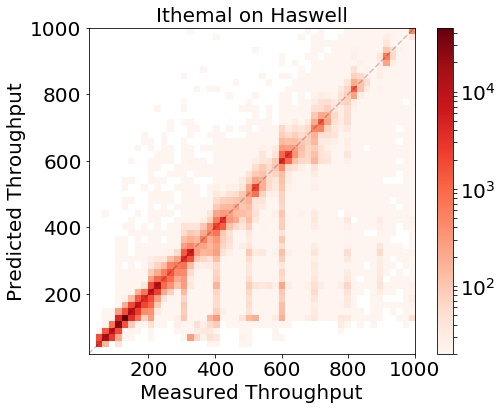
\includegraphics[width=0.33\textwidth]{figures/heatmap_ithemal_haswell.png}
	}
	\subfloat[][llvm-mca]{
		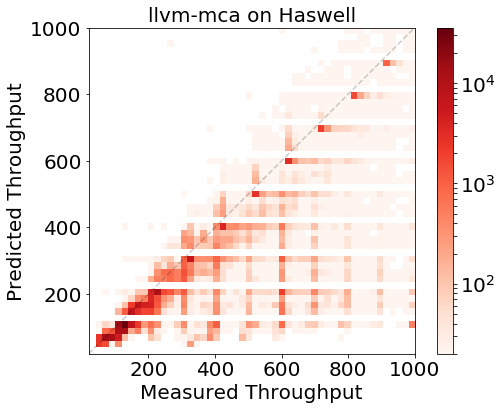
\includegraphics[width=0.33\textwidth]{figures/heatmap_llvm_haswell.png}
	}
	\subfloat[][IACA]{
		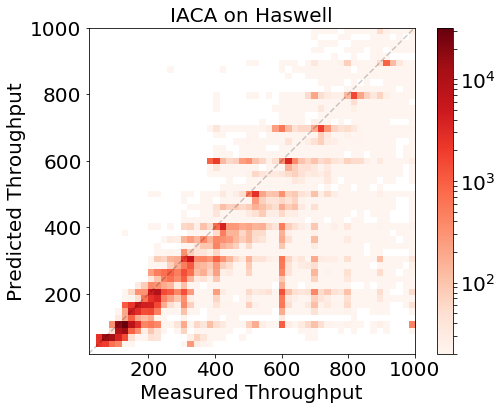
\includegraphics[width=0.33\textwidth]{figures/heatmap_iaca_haswell.png}
	}

	\caption{Heatmaps for measured and predicted throughput values under different models for basic blocks with measured throughput values less than 1000 cycles (Haswell)}
	\label{fig:accuracy}
\end{figure*}


We have evaluated \tool{} against two state-of-the-art, hand-written analytical models: IACA~\cite{iaca} (v3.0-28-g1ba2cbb) and llvm-mca~\cite{llvm-mca} (LLVM 8.0.0).
Both of these models are designed to model the complexities of modern processors (including pipelining, superscalar, and out-of-order units).
We show that our data--driven model beats the accuracy of these sophisticated hand-written models (Section~\ref{sec:accuracy}) while maintaining just as fast prediction speeds (Section~\ref{sec:speed}).
Further, we show that our approach is portable across different microarchitectures in Section~\ref{sec:portability} by showing that \tool{} learns a model that outperforms IACA and llvm-mca without any neural network architecture or hyperparameter modifications.

\subsection{Accuracy}
\label{sec:accuracy}

We evaluate the accuracy of each model against the actual throughput values for Intel's Haswell, Ivy Bridge, and Skylake microarchitectures.
The version of IACA we use does not support throughput estimation for Ivy Bridge; we therefore evaluate accuracy only for \tool{} and llvm-mca for Ivy Bridge.
We prepared datasets for each microarchitecture according to the methodology described in Section~\ref{sec:training}.

Table~\ref{tbl:accuracy} presents the results of our accuracy comparison.
We report the average error with respect to the ground truth of each tool for each microarchitecture.
We also report both the Spearman and Pearson correlation of each tool's predictions with the ground truth.

\tool{} is more accurate in its throughput predictions for basic blocks across all three microarchitectures.
Our model's predictions are closer to the ground truth than both IACA and LLVM in 74\% of the blocks in the Haswell test set.
\tool{}'s predictions also have a higher correlation with the ground truth values for both the Spearman (rank correlation) and Pearson (linear correlation) metrics.
The higher Spearman correlation is especially useful because it directly corresponds to higher utility for use within an optimizing compiler (such as an instruction scheduling pass).
Specifically, compilers typically only need to determine which of several configurations of a basic block is the fastest, and do not calculate each block's absolute performance.

Figure~\ref{fig:accuracy} presents three heatmaps relating actual and predicted values in for basic blocks with throughputs less than 1000 cycles for each prediction method (representing $95\%$ of our dataset).

To generate each heatmap, we binned the actual and predicted data into axis-aligned bins of width and height 20 cycles.
The color in each bin represents the count of blocks in that bin.
A perfect estimator would have all points along the line $y=x$ (shown as a faint grey, dashed line on the heatmaps), since the predicted throughputs would always match the measured throughputs.
We see a higher density near the identity line for \tool{}, compared to both llvm-mca and IACA.
Both llvm-mca and IACA also have more horizontal banding, representing more predictions of the same throughput value for different blocks that do actually have different behaviors.
Figure~\ref{fig:prederror} shows the average error of each system across a range of throughputs.
Compared to llvm-mca and IACA, \tool{} is better for blocks of almost all sizes.
All estimators struggle with blocks with measured throughputs just below peaks
in the measured throughput distribution. We hypothesize that these blocks correspond to special
microarchitectural optimizations that llvm-mca and IACA do not model. Ithemal also struggles
some with these rare blocks, but still outperforms both analytical estimators.

\begin{table}[h!]
  \small
  \begin{center}
    % \begin{tabular}{ |l|p{1.5cm}|C{2cm}|}
\begin{tabularx}{0.48\textwidth}{ |p{1.4cm}|l|l|C{1.5cm}|C{1.2cm}| }
  \hline
  Micro\-architecture & Method & Error & Spearman Correlation & Pearson Corr. \\
  \hline
  Ivy Bridge  & llvm-mca & 0.181 & 0.902 & 0.777 \\
              & \tool{}  & \textbf{0.089} & \textbf{0.955} & \textbf{0.913} \\
  \hline
  Haswell  & llvm-mca & 0.200 & 0.890 & 0.790 \\
           & IACA  & 0.209 & 0.917 & 0.833 \\%
           & \tool{}  & \textbf{0.089} & \textbf{0.960} & \textbf{0.918} \\
  \hline
  Skylake  & llvm-mca & 0.239 & 0.852 & 0.729 \\
           & IACA  &  0.167 & 0.926 & 0.835 \\
           & \tool{}  & \textbf{0.079} & \textbf{0.960} & \textbf{0.895} \\
  \hline
\end{tabularx}
  \end{center}
  \vspace{-10pt}
  \caption{Average error for different models and microarchitectures}
  \label{tbl:accuracy}
\end{table}

\begin{figure}[h!]
  \centering
  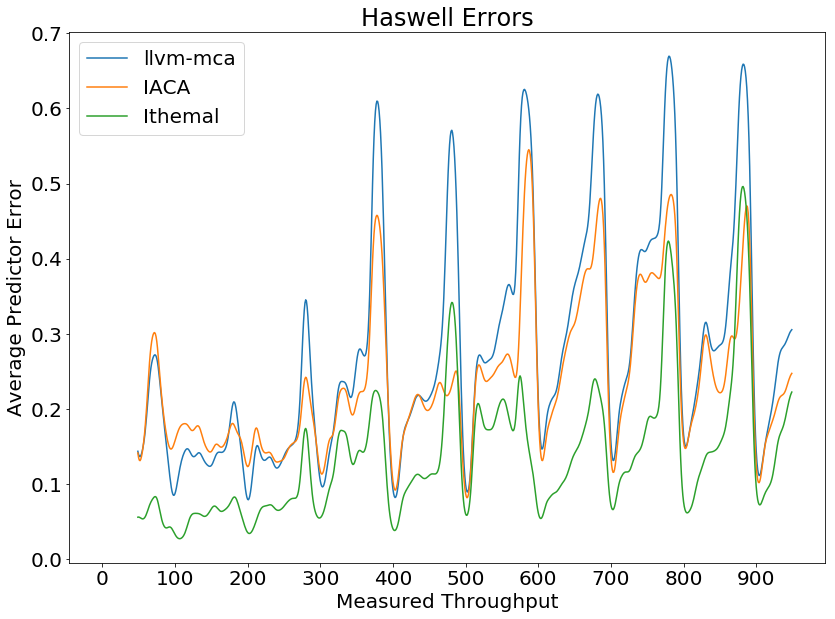
\includegraphics[width=\columnwidth]{figures/allsystems_errors_1.png}
  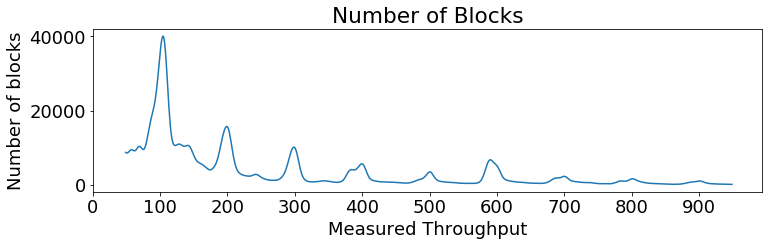
\includegraphics[width=\columnwidth]{figures/haswell_counts_short.png}
    \caption{Average error across throughputs for different estimation methods for basic blocks with throughput values less than 1000 cycles (Haswell)}
    \label{fig:prederror}
  \end{figure}

\subsection{Speed}
\label{sec:speed}

Table~\ref{tbl:speed} presents the results of our evaluation of \emph{estimator throughput}: the number of instructions able to be timed per second for each estimator.
We calculate this by measuring the number of basic blocks each tool can time per second, and multiplying that by the average number of instructions per basic block.
In the last row, we also show the corresponding estimator throughput if we instead measure the ground-truth throughput for a given block.
We measured these estimator throughputs on the Haswell test set on a machine with an Intel Xeon E5-2680 CPU.

\tool{} is as fast as llvm-mca and IACA in our measurements, and is significantly faster than empirical evaluation of basic blocks.
It is worth noting that llvm-mca and IACA can both also output diagnostic information about basic blocks, and also that empirical evaluation of ground-truth data could be sped up by running fewer repeated measurements (it may be possible that as few as 2 or 3 measurements would suffice in some contexts).
However even with these qualifications, we show that \tool{} functions as an equivalently performant and more accurate drop-in replacement for llvm-mca and IACA in systems which only need throughput estimations, while still performing significantly faster than empirical evaluation.

\begin{table}[h!]
  \small
  \begin{center}
\begin{tabular}{ |l|c| }
  \hline
  Method & Throughput (Instructions / second)  \\
  \hline
   llvm-mca & 492  \\  % 83.55 * 5.89
   IACA & 541  \\ % 91.92 * 5.89
   \tool{} & 560 \\ % 95.11 * 5.89
   Empirical execution & 13 \\ % 2.17 * 5.89
  \hline
\end{tabular}
  \end{center}
  \vspace{-10pt}

  \caption{Estimation throughputs for different estimators measured in instructions per second}
  \label{tbl:speed}
\end{table}

\subsection{Portability}
\label{sec:portability}

We designed and trained \tool{} on Haswell and validated our architecture and hyperparameters by re-training on Skylake.
Without any changes to its structure or training regime, we then trained and evaluated \tool{} on the Ivy Bridge dataset.
Table~\ref{tbl:accuracy} summarizes the average errors for each microarchitecture.
\tool{} learns to estimate throughput values for each microarchitecture with a maximum average error of 0.089 across all datasets.
The hand-written models exhibit a minimum average error of 0.167.

In sum, \tool{} provides state-of-the-art prediction performance; its results beat the baselines across the board.
Moreover, \tool{} does so without requiring a user to provide information about the processor's underlying microarchitecture, whereas these analytical models require significant re-engineering for each microarchitecture of interest.
